\let\negmedspace\undefined
\let\negthickspace\undefined
\documentclass[journal]{IEEEtran}
\usepackage[a5paper, margin=10mm, onecolumn]{geometry}
%\usepackage{lmodern} % Ensure lmodern is loaded for pdflatex
\usepackage{tfrupee} % Include tfrupee package
\setlength{\headheight}{1cm} % Set the height of the header box
\setlength{\headsep}{0mm}     % Set the distance between the header box and the top of the text
\usepackage{gvv-book}
\usepackage{gvv}
\usepackage{cite}
\usepackage{amsmath,amssymb,amsfonts,amsthm}
\usepackage{algorithmic}
\usepackage{graphicx}
\usepackage{textcomp}
\usepackage{xcolor}
\usepackage{txfonts}
\usepackage{listings}
\usepackage{enumitem}
\usepackage{mathtools}
\usepackage{gensymb}
\usepackage{comment}
\usepackage[breaklinks=true]{hyperref}
\usepackage{tkz-euclide} 
\usepackage{listings}
% \usepackage{gvv}                                        
\def\inputGnumericTable{}                                 
\usepackage[latin1]{inputenc}                                
\usepackage{color}                                            
\usepackage{array}                                            
\usepackage{longtable}                                       
\usepackage{calc}                                             
\usepackage{multirow}                                         
\usepackage{hhline}                                           
\usepackage{ifthen}                                           
\usepackage{lscape}
\usepackage{circuitikz}
\tikzstyle{block} = [rectangle, draw, fill=blue!20, 
    text width=4em, text centered, rounded corners, minimum height=3em]
\tikzstyle{sum} = [draw, fill=blue!10, circle, minimum size=1cm, node distance=1.5cm]
\tikzstyle{input} = [coordinate]
\tikzstyle{output} = [coordinate]
\begin{document}
\bibliographystyle{IEEEtran}
\vspace{3cm}
\title{9.3.8}
\author{AI25BTECH11017-BALU}
 \maketitle
% \newpage
% \bigskip
{\let\newpage\relax\maketitle}
\renewcommand{\thefigure}{\theenumi}
\renewcommand{\thetable}{\theenumi}
\setlength{\intextsep}{10pt} % Space between text and floats
\numberwithin{equation}{enumi}
\numberwithin{figure}{enumi}
\renewcommand{\thetable}{\theenumi}
\textbf{Question}:\\
Find the area of the region $\{(x, y) : x^2 \leq y \leq x\}$.
\\
\solution \\
Let us solve the given equation theoretically and then verify the solution computationally \\
According to the question, \\
equation line
\begin{align}
\vec{x}=\lambda\myvec{1\\1}
\end{align}
equation of parabola is
\begin{align}
   \vec{x}^T\vec{v}\vec{x}+2\vec{u}^T\vec{x}+f=0
\end{align}
where
\begin{align}
   \vec{v}=\myvec{1&&0\\0&&0}\\
   \vec{u}=\myvec{0\\\frac{-1}{2}}\\
   f=0
\end{align}
substute 0.1 in 0.2\\
$\lambda=0,1$ so intersection points are
\begin{align}
   \vec{a_1}=\myvec{0\\0}\\
   \vec{a_2}=\myvec{1\\1}\
\end{align}
hence the requried area is
\begin{align}
    \int_{0}^{1} (x-x^2) \, dx=\frac{1}{6}
\end{align}
\begin{figure}
    \centering
    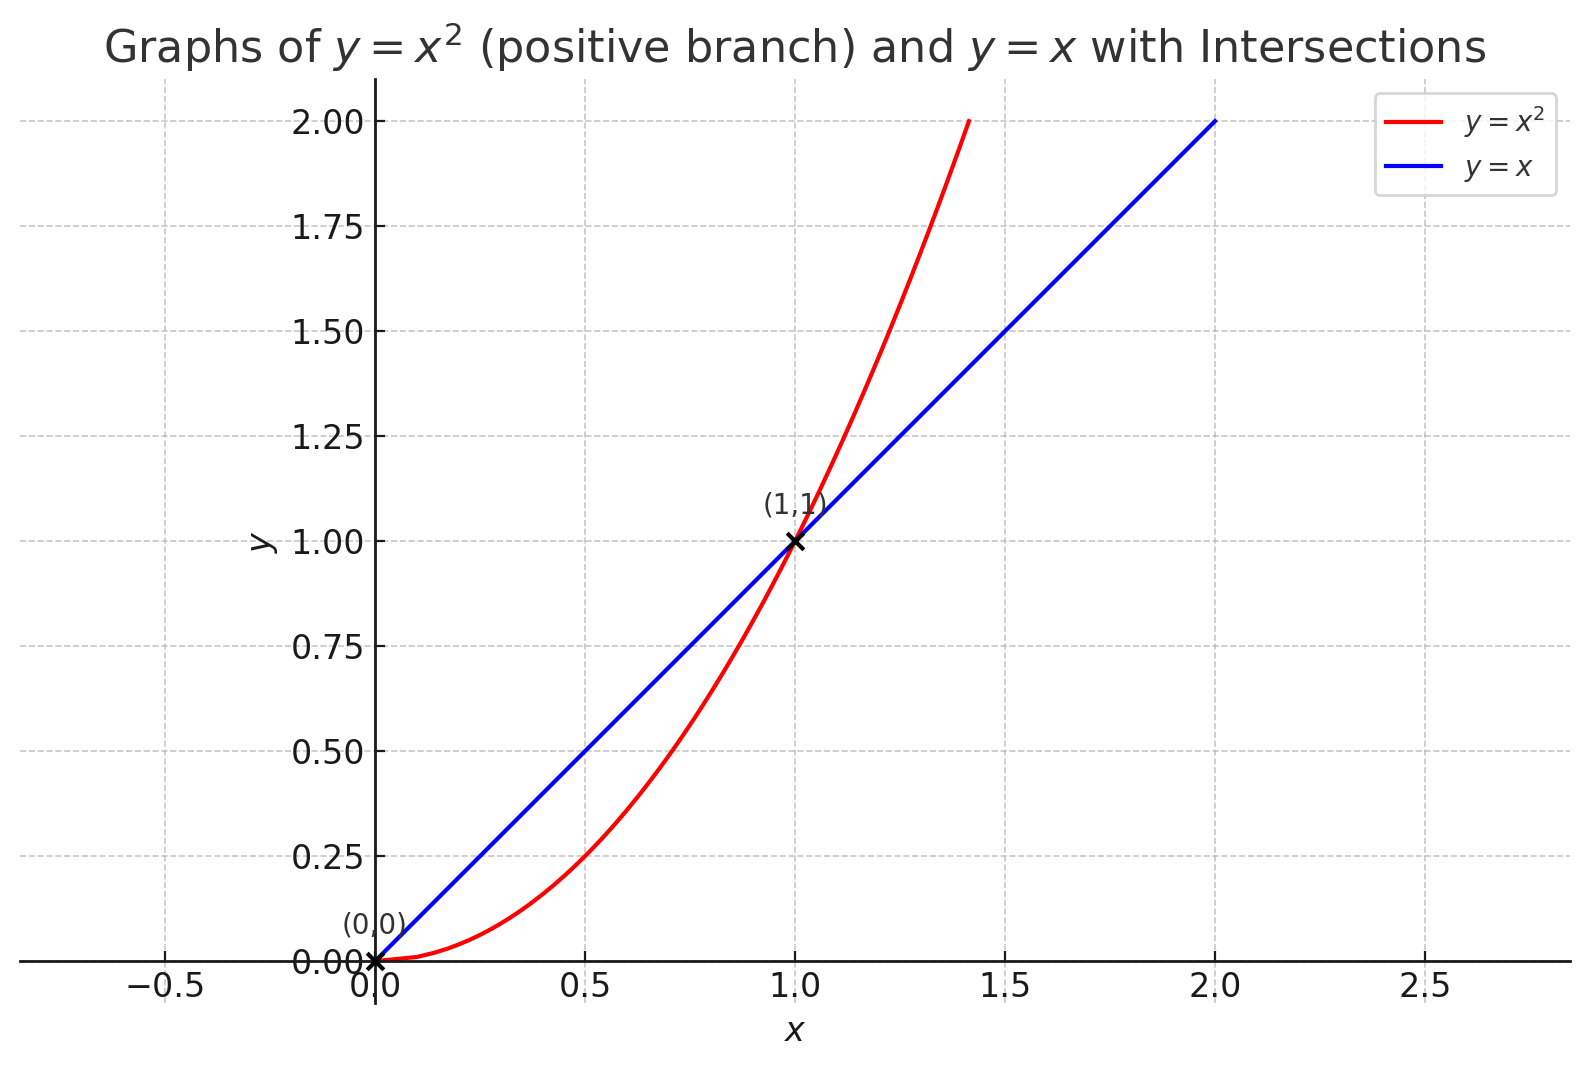
\includegraphics[width=0.5\linewidth]{figs/parabola_line.png}
    \caption{}
    \label{fig:placeholder}
\end{figure}
\end{document}